\subsection{Tipo de entidad Reunión}

   \begin{description}

   \item[Definición] Se refiere al objeto del mundo real: \emph{``Encuentro,
   real o virtual, entre un usuario asesor y al menos un usuario alumno''}.

   \item[Características] La entidad presenta las siguientes características:
      \begin{itemize}
         \item \textbf{Nombre:} Pregunta Asesor.
         \item \textbf{Tipo:} Débil por identificación con respecto a
         Alumno Curso Académico.
         \item \textbf{Número de atributos:} 3 propios y 2 heredados.
         \item \textbf{Atributo/s identificador/es principal/es:} dni\_pasaporte
         junto con curso\_académico e id\_reunión.
         \item \textbf{Atributo/s identificador/es alternativo/s:} -
         \item \textbf{Atributo/s heredado/s:} dni\_pasaporte y curso\_académico
         del tipo de entidad Alumno Curso Académico.
      \end{itemize}

   \item[Diagrama] La figura \ref{diagramaReunion} muestra el diagrama de la entidad.
   \item \begin{figure}[!ht]
            \begin{center}
            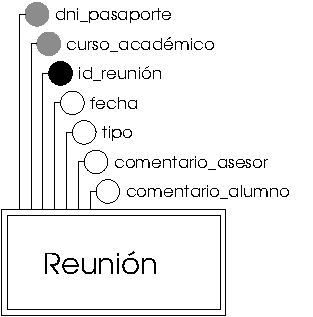
\includegraphics[]{07.Modelo_Entidad-Interrelacion/7.2.Analisis_Entidades/diagramas/reunion.pdf}
            \caption{Diagrama de la entidad Reunión.}
            \label{diagramaReunion}
            \end{center}
         \end{figure}

   \item[Descripción de los atributos propios] La entidad presenta los siguientes
   atributos propios:

   \begin{itemize}
    \item \textbf{id\_reunión}
      \begin{itemize}
         \item \textbf{Definición:} Código que sirve como número identificativo
               para cada reunión del sistema.
         \item \textbf{Dominio:} Números naturales.
         \item \textbf{Carácter:} Obligatorio.
         \item \textbf{Ejemplo práctico:} 121.
         \item \textbf{Información adicional:} El dato lo genera el sistema
               cuando se introduce una nueva reunión en el sistema. Es la clave
               primaria.
      \end{itemize}
   \item \textbf{fecha}
          \begin{itemize}
            \item \textbf{Definición:} Establece el día, mes y año cuando se
            produce la reunión.
            \item \textbf{Dominio:} Formato de fecha: dd/mm/aaaa.
            \item \textbf{Carácter:} Opcional.
            \item \textbf{Ejemplo práctico:} 01/01/2009.
            \item \textbf{Información adicional:} El dato lo introduce el
            usuario asesor cuando introduce una nueva reunión en el sistema.
         \end{itemize}
   \item \textbf{tipo}
          \begin{itemize}
            \item \textbf{Definición:} Establece el tipo de reunión realizada,
            ya sea grupal o individual.
            \item \textbf{Dominio:} Unos de los valores: grupal o individual.
            \item \textbf{Carácter:} Obligatorio.
            \item \textbf{Ejemplo práctico:} Individual.
            \item \textbf{Información adicional:} El dato lo introduce el
            usuario asesor cuando introduce una nueva reunión en el sistema.
         \end{itemize}
   \end{itemize}

   \item[Ejemplo práctico]

   \item \begin{center}
            \begin{tabular}{ | l | l | }
            \hline
            \multicolumn{2}{ | c | }{\textbf{Tipo de entidad Reunión}} \\
            \hline
            dni\_pasaporte & 01234567A \\
            \hline
            curso\_académico & 2008 \\
            \hline
            id\_reunión & 121 \\
            \hline
            fecha & 01/01/2009 \\
            \hline
            tipo & Individual \\
            \hline
            \end{tabular}
         \end{center}
   \end{description}
